\documentclass[ngerman, 12pt, pdftex]{scrartcl}[2006/07/30]

%encoding and input
\usepackage[ngerman]{babel} %spell correction
\usepackage[utf8]{inputenc} 
\usepackage[T1]{fontenc}

%bugfixes
\usepackage{fixltx2e} 

%Font Symbols and Colors
\usepackage{textcomp} %more symbols
\usepackage{xcolor}
\usepackage{hyperref}

%Math
\usepackage{amsmath}
\usepackage{mathtools} %extends amsmath

%Programming
\usepackage{listingsutf8} %in utf8
\lstset{language=Java,captionpos=b,tabsize=3,frame=,keywordstyle=\color{blue},commentstyle=\color{teal},stringstyle=\color{red},numbers=none,numberstyle=\tiny,numbersep=5pt,breaklines=false,showstringspaces=false,basicstyle=\footnotesize,emph={label},upquote=false} %Syntax highlighting

%Verbatim extension (with line numbers and tab-expansion)
\usepackage{moreverb} 

%Headers and Footer
\usepackage{fancyhdr}

%title
\title{Dokumentation}
\author{Frank M\"{u}ller, Oliver Wisler, Lucius Bachmann, Fabio Sulser}
\subtitle{Swissdefcon-Team}

\begin{document}
%declare  Header
\pagestyle{fancy}
\fancyhf{} 
\fancyhead[L]{Dokumentation} %left header
\fancyhead[C]{Swissdefcon-Team} %centered header
\fancyhead[R]{\thepage}  % right header
\renewcommand{\headrulewidth}{0.1pt} 	%upper separating line
%\fancyfoot[C]{\thepage} 				%centered footer, line number



%you might want to enable come features:
\maketitle
%\listoffigures 
%\listoftables


\newpage

\tableofcontents

\newpage

\section{Grobaufbau}
Unser Projekt gliedert sich in 5 grosse Pakete, alle Klassen welche Client und Server übergreifend verwendet werden, 
befinden sich im Paket "shared". Der ganze Server befindet sich im Paket "server" und der Client im Paket "Client".
Zum Ausprobieren und testen während dem Programmieren, als auch für den Unittest gibt es das Paket "test".

%-- Client
\section{Client}
\subsection{Aufbau}
Der Client gliedert sich in 6 Pakete, wovon 4 der Datenverwaltung dienen und 2 jeweils für die Lobby oder das Spiel zuständig sind.
Eine kurze Beschreibung der Pakete findet sich in der folgenden Tabelle:
\begin{table}[h!]
\begin{tabular}{ l p{12cm} }
  Paketname & Zweck \\ \hline
  net &  stellt Klassen für die Kommunikation und Serversuche zur Verfügung. In diesem Paket werden alle empfangenen Daten ausgewertet und mittels Event oder statischen Funktionen weitergeleitet.\\
  events & Stellt Events zur Verfügung welche für die interne Kommunikation im Client genutzt werden. (GameEvent, ChatEvent)\\
  data&  haltet Daten welche für das Spiel oder die Lobby wichtig sind (die Spielerid, Zuordnung Spieler zu Id, etc...).\\
  resources & Stellt eine Klasse zur Verfügung mittels derer Daten (Bilder, etc...) geladen werden können.\\
  lobby & Beinhaltet die ganze Lobby\\
  game & Beinhaltet das GUI für das Spiel\\
\end{tabular}
\caption{Unterpakete im Paket client}
\end{table}
\begin{figure}[h!]
\centering
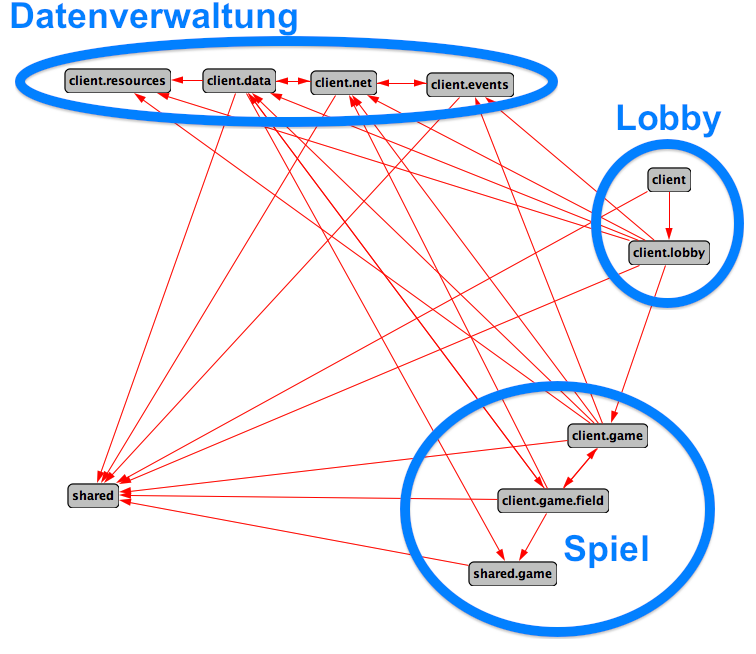
\includegraphics[scale=0.4]{client/client_aufbau_ann.png}
\caption{Importe zwischen den Paketen}
\end{figure}

\subsection{Datenverwaltung}
Ausgehend vom Parser werden die Daten mit zwei Methoden verteilt.
Daten welche nicht permanent gespeichert werden müssen (z.Bsp. Chatnachrichten) werden per Event 
weitergeleitet, so dass von überall her mit einem geeigneten Listener darauf zugegriffen werden kann.
Daten welche langfristig gespeichert werden (zum Beispiel die Zuordnung von Spielernamen zu ihrer Id) werden
von Klassen im Paket "client.data" gespeichert. Darunter fällt  "PlayerManager" welcher alle Informationen bezüglich Spieler speichert und "RunningGame" welche alle Informationen zum gerade laufenden Spiel bereithält.
Auf diese gespeicherten Daten kann mittels statischer Methoden jederzeit vom Spiel oder von der Lobby zugegriffen werden.
frank
\begin{figure}[h!]
\centering
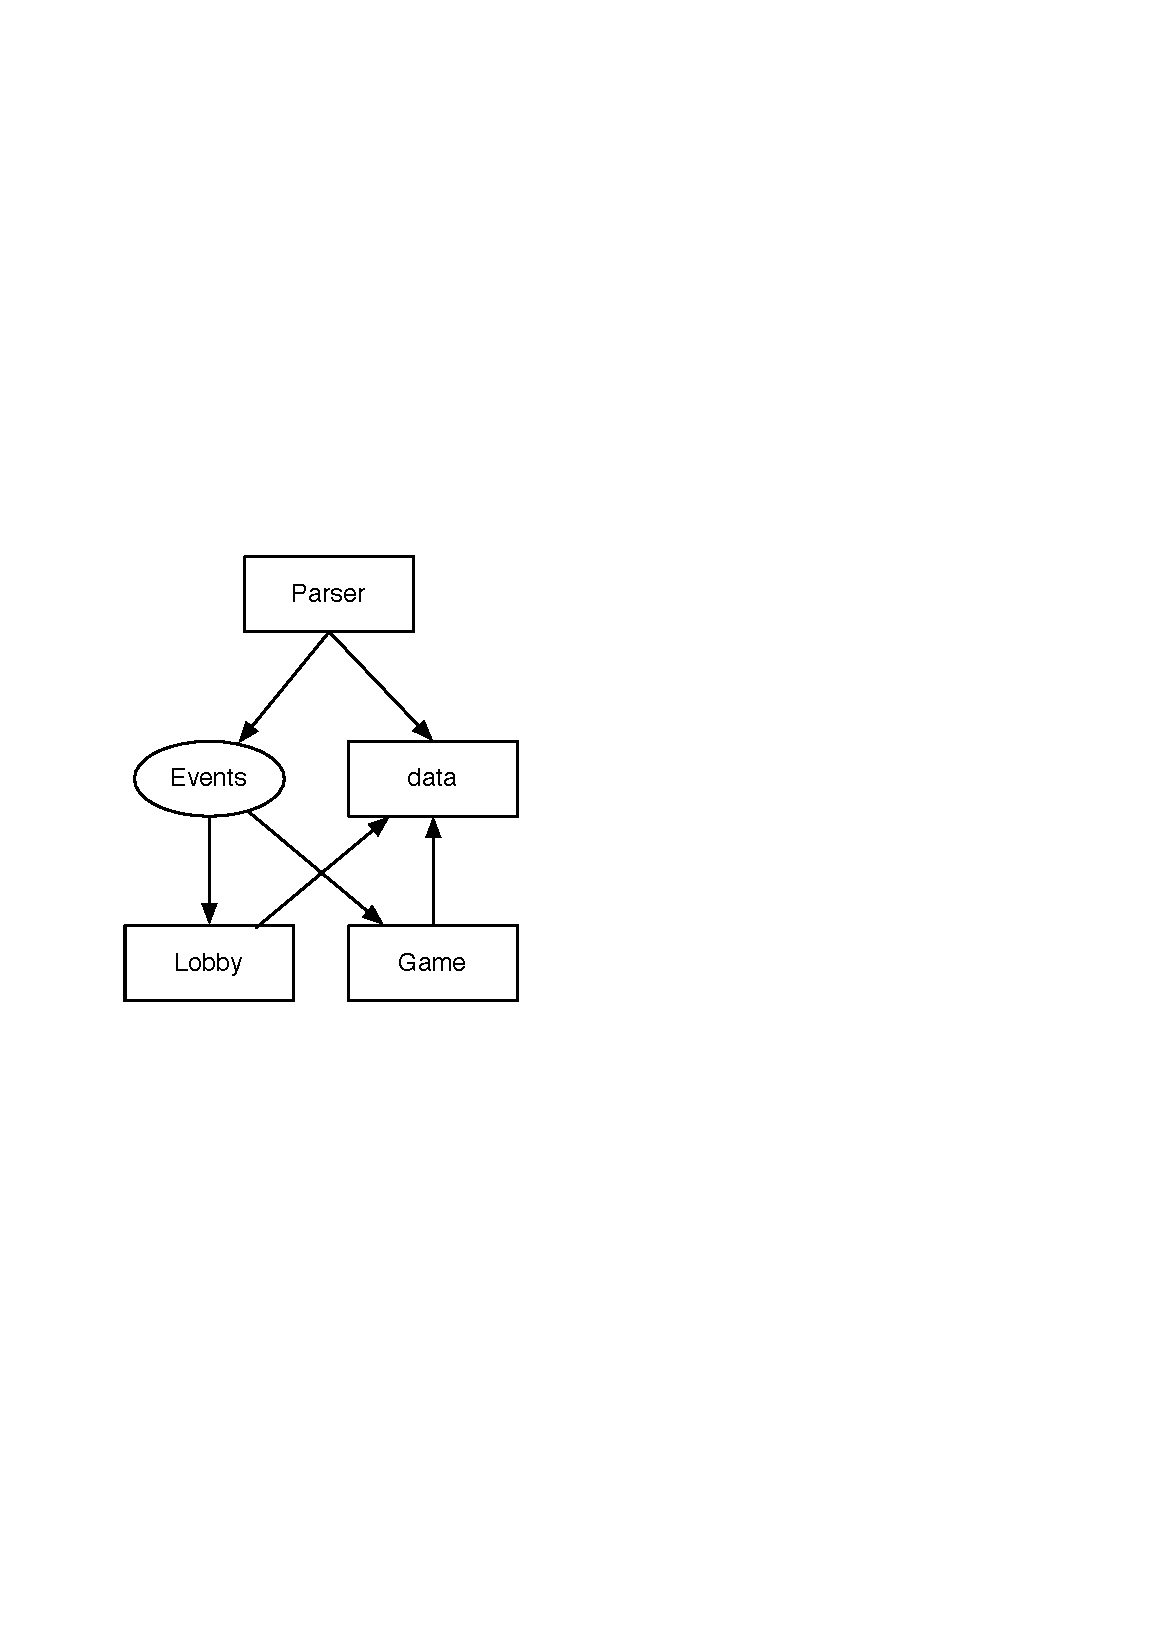
\includegraphics[scale=0.6]{client/datenhaltung.pdf}
\caption{Datenverteilung}
\end{figure}

\subsection{Rendering}

Das Ganze Bild wird über einen doubleBuffer gezeichnet.
Dazu wird aufgrund der Bildschirmgr\"{o}sse die optimale Spielfeldgr\"{o}sse ermittelt.
Die gesetzten Objekte werden gezeichnet, fals sie bewegt wurden, wird eine Linie und eine Pfeilspitze mit Referenz auf das Objekt gezeichnet.
Ein Algorithmus \"{u}berpr\"{u}ft, ob bei einem Klick auf ein Objekt gedr\"{u}ckt wurde oder nicht. Falls nein, wird ein neues Objekt an der gedr\"{u}kten Stelle gezeichnet, ansonsents wird die moving-range, sowie Lebenspunkte und aktuellen Wert des angew\"{a}hlten Objektes auf dem Spielfeld angezeigt.
Die h\"{a}ufigkeit, in der das Spielfeld neu gezeichnet wird, h\"{a}ngt von der Spielsituation ab. Ist ein Objekt angew\"{a}hlt, so wird das Bild alle 70 Millisekunden neu gezeichnet. Ist kein Objekt angew\"{a}hlt, so wird das Bild alle 200 Millisekunden neu gezeichnet. In der Animationsphase wird das Bild alle 20 Millisekunden neu erstellt.
Wird die Gr\"{o}sse des Fenster ver\"{ä}ndert, so wird das Bild neu gerendert.
Die Objekte werden als Bild gezeichnet und farbig umrandet. Jeder Spieler besitz auf der gegnerischen Karte eine andere Farbe, seine eigene ist jedoch immer Blau.
Der Radar wird als dreieckige Polygone gezeichnet, die mit dem zunehmenden Winkel an Farbe verlieren. Die Objektangaben werden als Strings gezeichnet.


%-- Server
\section{Server}
\subsection{Aufbau}
Der Server gliedert sich in 9 Pakete, wovon 4 der Datenverwaltung dienen. Die andern Pakete enthalten Serverinterne Exceptions, das GUI, die Spiellogik und das Socket.
Eine kurze Beschreibung der Pakete findet sich in der folgenden Tabelle:
\begin{table}[h!]
\begin{tabular}{ l p{11.5cm} }
  Paketname & Zweck \\ \hline
  
  net &  
  Stellt Klassen für die Kommunikation und Serversuche zur Verfügung. \\
  
  exceptions & 
  Hält Serverinterne Exceptions\\
  
  GamePlayObjects &
  Hält alle Objekte, die gebaut werden können (Bomber, Jets, Banken, usw.)\\
  
  logic &
  Hält die Spiellogik, die die Runden bestimmt und überprüft.\\
  
  parser &
  In diesem Paket werden alle empfangenen Daten ausgewertet und die Saten an die jeweiligen Funktionen übergeben.\\
  
  players &
  Hält alle Spielerbezogenen Daten. (Name, ID, Socket, Server, ...)\\
  
  score &
  Speichert eine Top-Ten der Spieler, die jederzeit aus der Lobby aufgerufen werden kann.\\
  
  server &
  Hält alle aktiven Spiele.\\
  
  UI &
  Hält das Benutzerinterface des Servers.\\
  
 
\end{tabular}
\caption{Unterpakete im Paket server}
\end{table}

\subsection{Datenverwaltung}
Die vom Parser empfangenen Daten werden aufgeteilt zu Spielerdaten, Objektdaten und Serverdaten.
Spielerdaten werden in der Instanz einer Player-Klasse des jeweiligen Spieler gespeichert. Objektdaten werden in der jeweiligen Instanz diese Objektes gespeichert. Serverdaten werden in einer Instanz der Server-Klasse gespeichert. Aktive Server werden vom Servermanager gehalten. Dieser entfernt auch automatisch inaktive Instanzen. 1
\begin{figure}[h!]
\centering
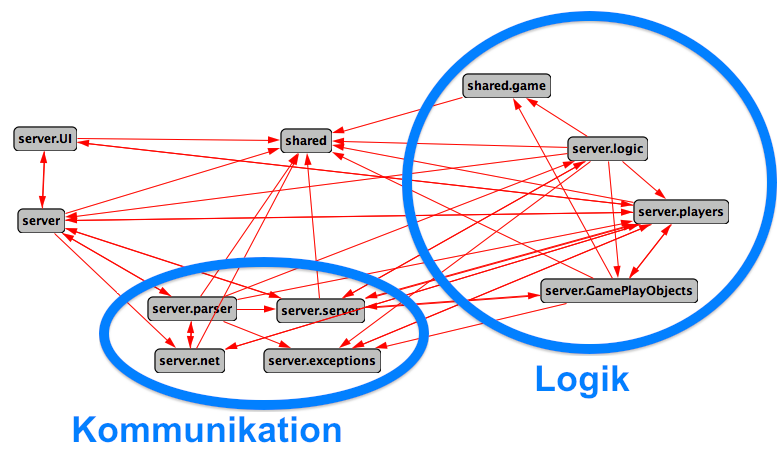
\includegraphics[width=14cm]{server/server.png}
\caption{Datenverteilung}
\end{figure}

\subsection{Spiellogik}
\subsubsection{Aufbauphase}
Mit dem Start des Spiels wird der GamePlayObjectManager instanziert. Er verwaltet die GamePlayObjects.
Wird ein Objekt erstellt, \"{u}bergibt man dem Objekt den GamePlayObjectManager. Das Objekt, falls es an einer g\"{u}ltigen Position gesetzt wurde und der Spieler noch Geld hat, tr\"{a}gt sich dann in die Liste AllObjects und, lalalalwenn ein Defensivobjekt, in die Liste Defensives ein. Wird ein Objekt bewegt, dann wird das in die Membervariable Target eingetragen.

\subsubsection{Runde}

Wird jetzt die Runde gestartet, dann..
\begin{itemize}

\item Testet der GamePlayObjectManager zuerst, ob ein Spieler noch Population hat. Wenn nicht, werden all seine Objekte gel\"{o}scht und sein Geld auf 0 gesetzt.
\item Darauf werden die Objekte gepr\"{u}ft, ob sie noch Lebenspunkte haben. Wenn nicht, werden sie gel\"{o}scht.
\item Dann rechnet jedes Objekt aus, wohin es sich bewegen wird. Falls ein Objekt weiter als seine MovingRange bewegt werden sollte, dann bewegt es sich in Richtung Target soweit, wie es die MovingRange erlaubt. Das Ergebnis wird in moveProv gespeichert.
\item Jetzt senden alle Objekte allen Objekten ihre Bewegung, und jedes Objekt testet die eingegangenen Bewegungen darauf, ob sie durch ihren Angriffsradius verlaufen. Wenn ja und angreifbar, werden sie in der Liste possibleTargets gespeichert. Dann werden die Objekte auf ihre neue Position gesetzt.
\item Schiesslich f\"{u}hren alle Objekte ihre Angriffe aus. Die Banken geben Geld, die Reproduktionszentren Bev\"{o}lkerung. Alle anderen Objekte w\"{a}hlen zuf\"{u}llig ein Objekt aus den possibleTargets aus, schiessen darauf bis es keine Lebenspunkte mehr hat, wenn es 0 Lebenspunkte hat w\"{a}hlen sie das n\"{a}chste Objekt, bis sie keine Munition mehr haben.
\end{itemize}



%-- Kommunikation
\section{Kommunikation}
\subsection{Serverauswahl}
Die Serverauswahl wird durch ein äusserst rudimentäres Discovery over Multicast bereitgestellt. Der Server sendet hier in konstantem Zeitabstand ein Multicast-Paket ins Netzwerk, das seinen Port enthält und natürlich auch seine IP (durch UDP-Packet-Header). Diese Lösung erfüllz zwar seinen Zweck, kann aber zu unnötigem Traffic innerhalb eines Netzwerkes führen. Dies zu verbessern wäre etwas für zukünftige Releases.

\subsection{Verbindung}
Die Verbindung basiert auf einem TCP-Socket beim Clienten und einem beim Server. Daher auf jedem Socket zwei Threads laufen (einer, der nur empfängt und einer, der nur sendet) können jederzeit daten gesendet und empfangen werden. Dies ermöglicht dem Server auch in Anwesenheit eines Routers jederzeit und instant, Nachrichten zum Clienten zu pushen. Das Socket beim Clienten sendet automatisch ein Ping, falls in den vorhergehenden 500ms keine Daten versendet wurden.


\subsection{Protokoll}
\subsubsection{Aufbau}
Jeder Protokolbefehl besteht aus 5 Buchstaben. Der erste Buchstaben bezeichnet jeweils den Bereich des Befehls, es sind dies:
\begin{itemize}
\item D für die Serversuche
\item V für Befehle betreffend der Verbindung
\item C für den Chat
\item G für das Spiel
\end{itemize}
\subsubsection{Befehle}
Alle Protokolbefehle können im Wiki unter \url{http://chaos-theory.ch/CS108/wiki/doku.php?id=protocol} abgerufen werden.

\section{Andere Pakete}
\subsection{shared}
Hier sind diverse Klassen, welche sowohl vom Server als auch vom Client benutzt werden.
Darunter fällt das Protokoll, ein InputValidator, welcher Eingaben validieren kann, Eine Klasse welche Log Funktionen zur Verfügung stellt,
diverse Einstellungen (Spiel und Kommunikation).

\section{Unittest}
\subsection{Die Klasse}
Funktionen der Klasse Bank:
\begin{itemize}
\item Der Konstruktor: 
\subitem Wenn der Spieler zuwenig Geld hat-> throw GameObjectBuildException
\subitem Wenn der Spieler das Objekt nicht in seinem Feld setzt-> throw GameObjectBuildException
\subitem Wenn der Spieler genug Geld hat und das Objekt in seinem Feld setzen will-> F\"{u}ge dich in die Liste aller GamePlayObjects vom Server ein.
\item die Methode damage(int damPoints)
\subitem Reduziere die Healthpoints um damPoints
\item Die Methode attack()
\subitem F\"{u}ge dem Besitzer das soviel Geld hinzu, wie in den Settings definiert.
\end{itemize}

\subsection{Der Test}
Getestet wurde:
\begin{itemize}
\item Ob es eine Exception gibt, wenn man eine Bank ohne Geld an ausserhalb des eigenen Feldes setzt. Wenn ja, ok, Wenn nein, fail.
\item Ob es eine Exception gibt, wenn man eine Bank ohne Geld an innerhalb des eigenen Feldes setzt. Wenn ja, ok, Wenn nein, fail.
\item Ob es eine Exception gibt, wenn man eine Bank ohne Geld an ausserhalb des eigenen Feldes setzt. Wenn ja, ok, Wenn nein, fail.
\item Ob es eine Exception gibt, wenn man eine Bank mit Geld an ausserhalb des eigenen Feldes setzt. Wenn ja, ok, Wenn nein, fail.
\item Ob es eine Exception gibt, wenn man eine Bank mit Geld an innerhalb des eigenen Feldes setzt.Wenn ja, fail, Wenn nein, ok.
\item Wenn die Bank korrekt erstellt wurde, ist sie dann in der Liste der Objekte: Wenn ja, ok, Wenn nein fail.
\item Wenn die Bank mit 100 Schadenspunkten besch\"{a}digt wurde, hat sie nacher 100 Healthpoints weniger. Wenn ja, ok, Wenn nein fail.
\item Wenn die attack Methode aufgerufen wurde, hat der Spieler soviel Geld mehr, wie in den Settings definiert? Wenn ja, ok, Wenn nein fail.
\end{itemize}

 

\end{document}